% !TEX root = task-1-10-3.tex
% Editable task bank. Append new BankTask blocks at the end of the document.
\documentclass[12pt,a4paper]{article}
\usepackage{physics-textbook}
\usepackage{graphicx,needspace}
\usetikzlibrary{decorations.pathmorphing}
\newif\ifShowSolutions
\ifdefined\TutorEdition
  \ShowSolutionstrue
\else
  \ShowSolutionsfalse % Change to \ShowSolutionstrue to display solutions.
\fi
\newcounter{banktask}
\newsavebox{\BankTaskBox}
\newcommand{\BankTaskContent}[3]{%
  \noindent\textbf{\thebanktask.}\quad #2\par
  \ifShowSolutions
    \Needspace{50mm}% Keep the solution heading with its opening text or diagram.
    #3\par
    \ifdefined\TutorEdition
      \ifcsname TutorSource#1\endcsname
        \nopagebreak\smallskip{\small\csname TutorSource#1\endcsname\par}%
      \fi
    \fi
  \fi
}
\newcommand{\BankTask}[3]{%
  \refstepcounter{banktask}\par\medskip
  \sbox{\BankTaskBox}{\begin{minipage}{\linewidth}%
    \BankTaskContent{#1}{#2}{#3}\end{minipage}}%
  \ifdim\dimexpr\ht\BankTaskBox+\dp\BankTaskBox\relax>\dimexpr\textheight-20mm\relax
    \Needspace{35mm}\BankTaskContent{#1}{#2}{#3}%
  \else
    \Needspace{\dimexpr\ht\BankTaskBox+\dp\BankTaskBox\relax}%
    \noindent\usebox{\BankTaskBox}\par
  \fi
  \medskip
}
\begin{document}
\BookSubsection{1.10.3}{Вес тела. Невесомость}


% Source 3A9974: https://ege.fipi.ru/bank/questions.php?search=1&proj=BA1F39653304A5B041B656915DC36B38&qid=3A9974
\BankTask{3A9974}{
Грузовик массой $10\,\text{т}$ проезжает верхнюю точку выпуклого моста, радиус кривизны которого равен $80\,\text{м}$, двигаясь равномерно со скоростью $72\,\text{км}/\text{ч}$.
\begin{enumerate}
\item Сила тяжести, действующая на грузовик, равна $10\,\text{кН}$.
\item Сумма сил, действующих на грузовик, направлена вертикально вверх и перпендикулярна его скорости.
\item Центростремительное ускорение грузовика равно $5\,\text{м}/\text{с}^{2}$.
\item Сила, с которой мост действует на грузовик, меньше $40\,\text{кН}$ и направлена вертикально вверх.
\item Сила, с которой грузовик действует на мост, направлена вертикально вниз и равна $50\,\text{кН}$.
\end{enumerate}
}{
\smallskip\noindent\textbf{Решение от GPT}\par
$m=10^4\,\text{кг}$, $v=20\,\text{м}/\text{с}$. Ускорение $a=v^2/R=5\,\text{м}/\text{с}^2$ направлено вниз. $mg=100\,\text{кН}$, $N=m(g-a)=50\,\text{кН}$ направлена вверх; на мост грузовик действует вниз с той же силой. Ответ: $35$.
}

% Source 7D140C: https://ege.fipi.ru/bank/questions.php?search=1&proj=BA1F39653304A5B041B656915DC36B38&qid=7D140C
\BankTask{7D140C}{
Мальчик поднимает вверх гирю массой $10\,\text{кг}$, действуя на неё постоянной силой $120\,\text{Н}$, направленной вертикально вверх.
\begin{enumerate}
\item Вес гири равен $120\,\text{Н}$ и направлен вверх.
\item Гиря действует на руку мальчика с силой $100\,\text{Н}$, направленной вниз.
\item Равнодействующая сил, действующих на гирю, равна $240\,\text{Н}$ и направлена вверх.
\item Ускорение гири равно $2\,\text{м}/\text{с}^{2}$.
\item Если мальчик приложит к гире направленную вертикально силу $90\,\text{Н}$, он не сможет её поднять.
\end{enumerate}
}{
\smallskip\noindent\textbf{Решение от GPT}\par
$mg=100\,\text{Н}$, $F_{\text{рез}}=120-100=20\,\text{Н}$ вверх, $a=20/10=2\,\text{м}/\text{с}^2$. Гиря действует на руку вниз с силой $120\,\text{Н}$. Сила $90\,\text{Н}<mg$ не позволяет поднять гирю из покоя. Ответ: $45$.
}

% Source 72C2B7: https://ege.fipi.ru/bank/questions.php?search=1&proj=BA1F39653304A5B041B656915DC36B38&qid=72C2B7
\BankTask{72C2B7}{
При помощи динамометра определяют вес металлической детали. Определите показание динамометра, если погрешность прямого измерения равна цене деления динамометра. Шкала проградуирована в $\text{Н}$.
\begin{center}
\par\begin{center}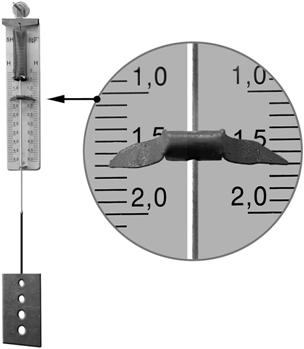
\includegraphics[width=.9\linewidth,height=.48\textheight,keepaspectratio]{_run/photos/1ea90dd9e3195991b9886d0a000478ef743ddaf9eaf6f3a83d7befae3e079b31.png}\end{center}\par
\end{center}
}{
\smallskip\noindent\textbf{Решение от GPT}\par
Между отметками $1{,}0$ и $1{,}5\,\text{Н}$ пять делений, поэтому цена деления равна $0{,}1\,\text{Н}$. Указатель соответствует $1{,}6\,\text{Н}$. Показание с учётом погрешности: $P=(1{,}6\pm0{,}1)\,\text{Н}$.
}

\end{document}
